% Preamble
\documentclass[11pt]{report}

% Packages
\usepackage[a4paper]{geometry}
\usepackage[english]{babel}
\usepackage[backend=biber,style=ieee]{biblatex}
\usepackage{hyphenat}
\usepackage{csquotes}
\usepackage[indent=20pt]{parskip}
\usepackage{hyperref}
\usepackage{graphicx}
\usepackage{listings}
\usepackage{subfiles}
\usepackage[table,xcdraw]{xcolor}
\usepackage[normalem]{ulem}
\usepackage{colortbl}
\usepackage{float}
\usepackage{booktabs}
\usepackage{tcolorbox}
\usepackage{aaufrontmatter}

% textidote: ignore begin
\useunder{\uline}{\ul}{}
% textidote: ignore end

% textidote: ignore begin

% Bibliography

% Configuration
\graphicspath{ {./images/} }

\hypersetup{pdfborder=0 0 0}

% textidote: ignore end

% Document
\title{}
\subtitle{}
\theme{Software Engineering}
\semester{Autumn}
\groupnumber{6}
\groupmembers{
    Kristiyan Mariyan Georgiev,
    Mads Heilmann,
    Martin Kedmenec,
    Sebastian Hemmer Bech Mygind,
    Simon Woidemann,
    Freja Johannesen
}
\supervisors{Tung Kieu}
\department{Software}
\abstract{}

\begin{document}
    % Title
    \maketitle

    % Table of Contents
    % textidote: ignore begin
    \tableofcontents
    % textidote: ignore end

    % Commenting out until it's ready
    % \makeaaupreface{This is the preface.}

    % Main Content
    \input{codestyling/java}

    % textidote: ignore begin
\section{Introduction}\label{sec:introduction}
% textidote: ignore end

    % textidote: ignore begin
\chapter{Problem analysis}\label{ch:problem-analysis}
% textidote: ignore end

% textidote: ignore begin
\subsection{State of the Art}\label{subsec:state-of-the-art}
% textidote: ignore end

The following section will look at and analyze existing solutions and their approach to visualizing statistics and
analytics, while looking for inspirations or areas to improve upon.
The chosen solutions are~\acrlong{ga4} and Microsoft BI, as they are both widely used for commercial purposes and
provide a wide range of features.
% TODO change microsoft bi to a different analytics tool that could fit better for the solution

\subsubsection{Google Analytics}\label{subsubsec:google-analytics}

% textidote: ignore begin % textidote doesn't like it when sentences start with acronyms
\acrfull{ga4} is a general purpose analytics tool that can provide data on a wide range of services, such as websites,
online stores, and mobile applications~\cite{ga4}.
% textidote: ignore end
Its main highlights are the ability to track website views, store sales, user interactions, and much more data.
% textidote: ignore begin
\acrshort{ga4} is also highly customizable, allowing a manager to create custom fields and metrics, as well as custom
reports and dashboards.
% textidote: ignore end
The main purpose of~\acrshort{ga4} is to help businesses with their marketing strategies, by providing data on user
behavior and demographics, as well as tracking the effectiveness of marketing campaigns.

\begin{figure}[H]
    \centering
    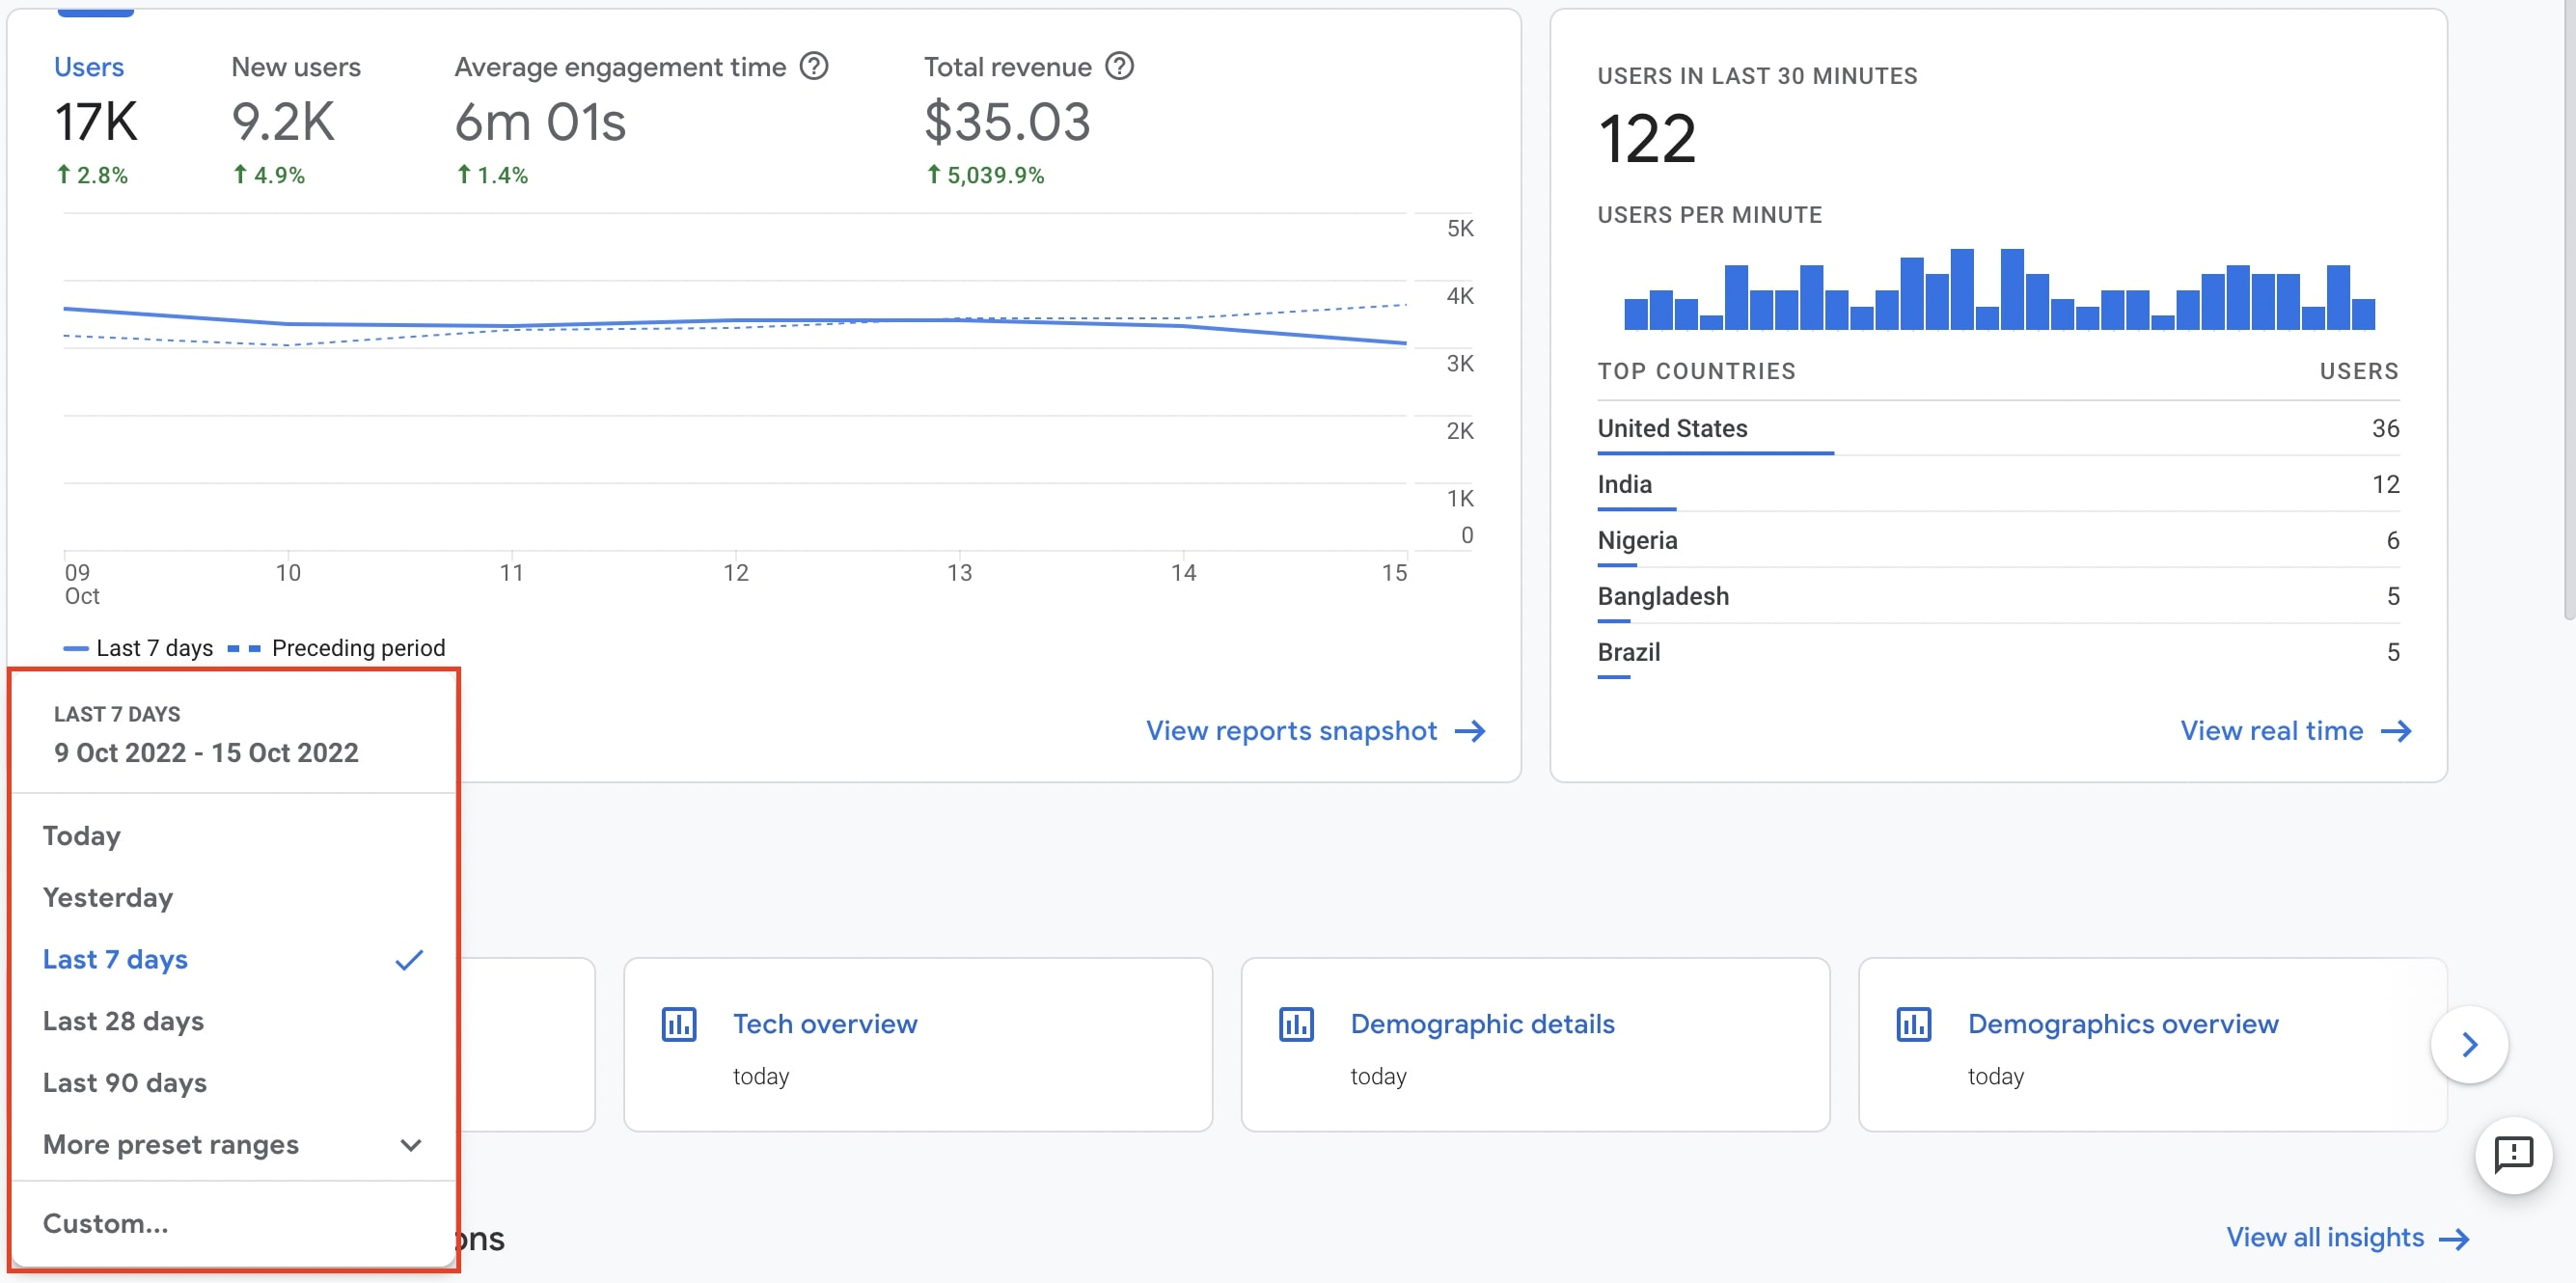
\includegraphics[width=1\textwidth]{problem-analysis/GA4-home}
    \caption{\acrshort{ga4} home dashboard.
    }\label{fig:GA4-dashboard}
\end{figure}

\begin{figure}[H]
    \centering
    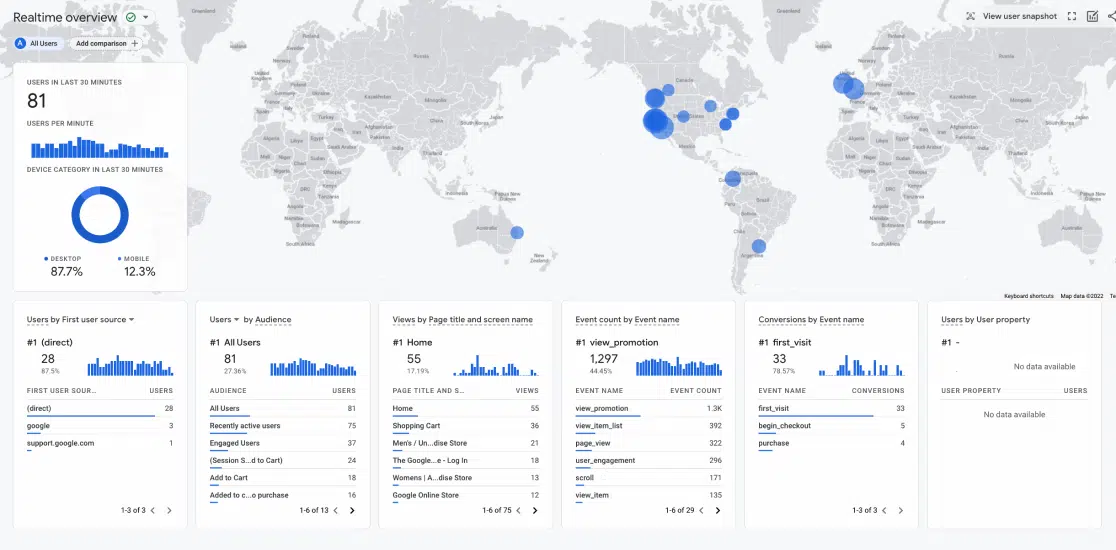
\includegraphics[width=1\textwidth]{problem-analysis/GA4-realtime}
    \caption{\acrshort{ga4} real-time page.
    }\label{fig:GA4-realtime}
\end{figure}

Figure~\ref{fig:GA4-dashboard} shows an example of the home dashboard in \acrshort{ga4}~\cite{ga4-interface}.
It is the first page the manager sees when logging in, and it provides an overview of the most important data.
The left side of the screen shows site activity in the last 7 days, but the graph can be changed to any time period.
The right side shows the number of users in the last 30 minutes, broken down to users per minute.
It's an elementary interface, but the power of~\acrshort{ga4} lies deeper in the menus.

Figure~\ref{fig:GA4-realtime} shows an example of the real-time page in \acrshort{ga4}~\cite{ga4-realtime}.
This is a powerful tool that allows the manager to monitor the current activity of the site.
It shows a map with the locations of the users currently online and how they interact with the website.
This can be useful to monitor any changes caused by marketing campaigns, product launches or other events.

\begin{figure}[H]
    \centering
    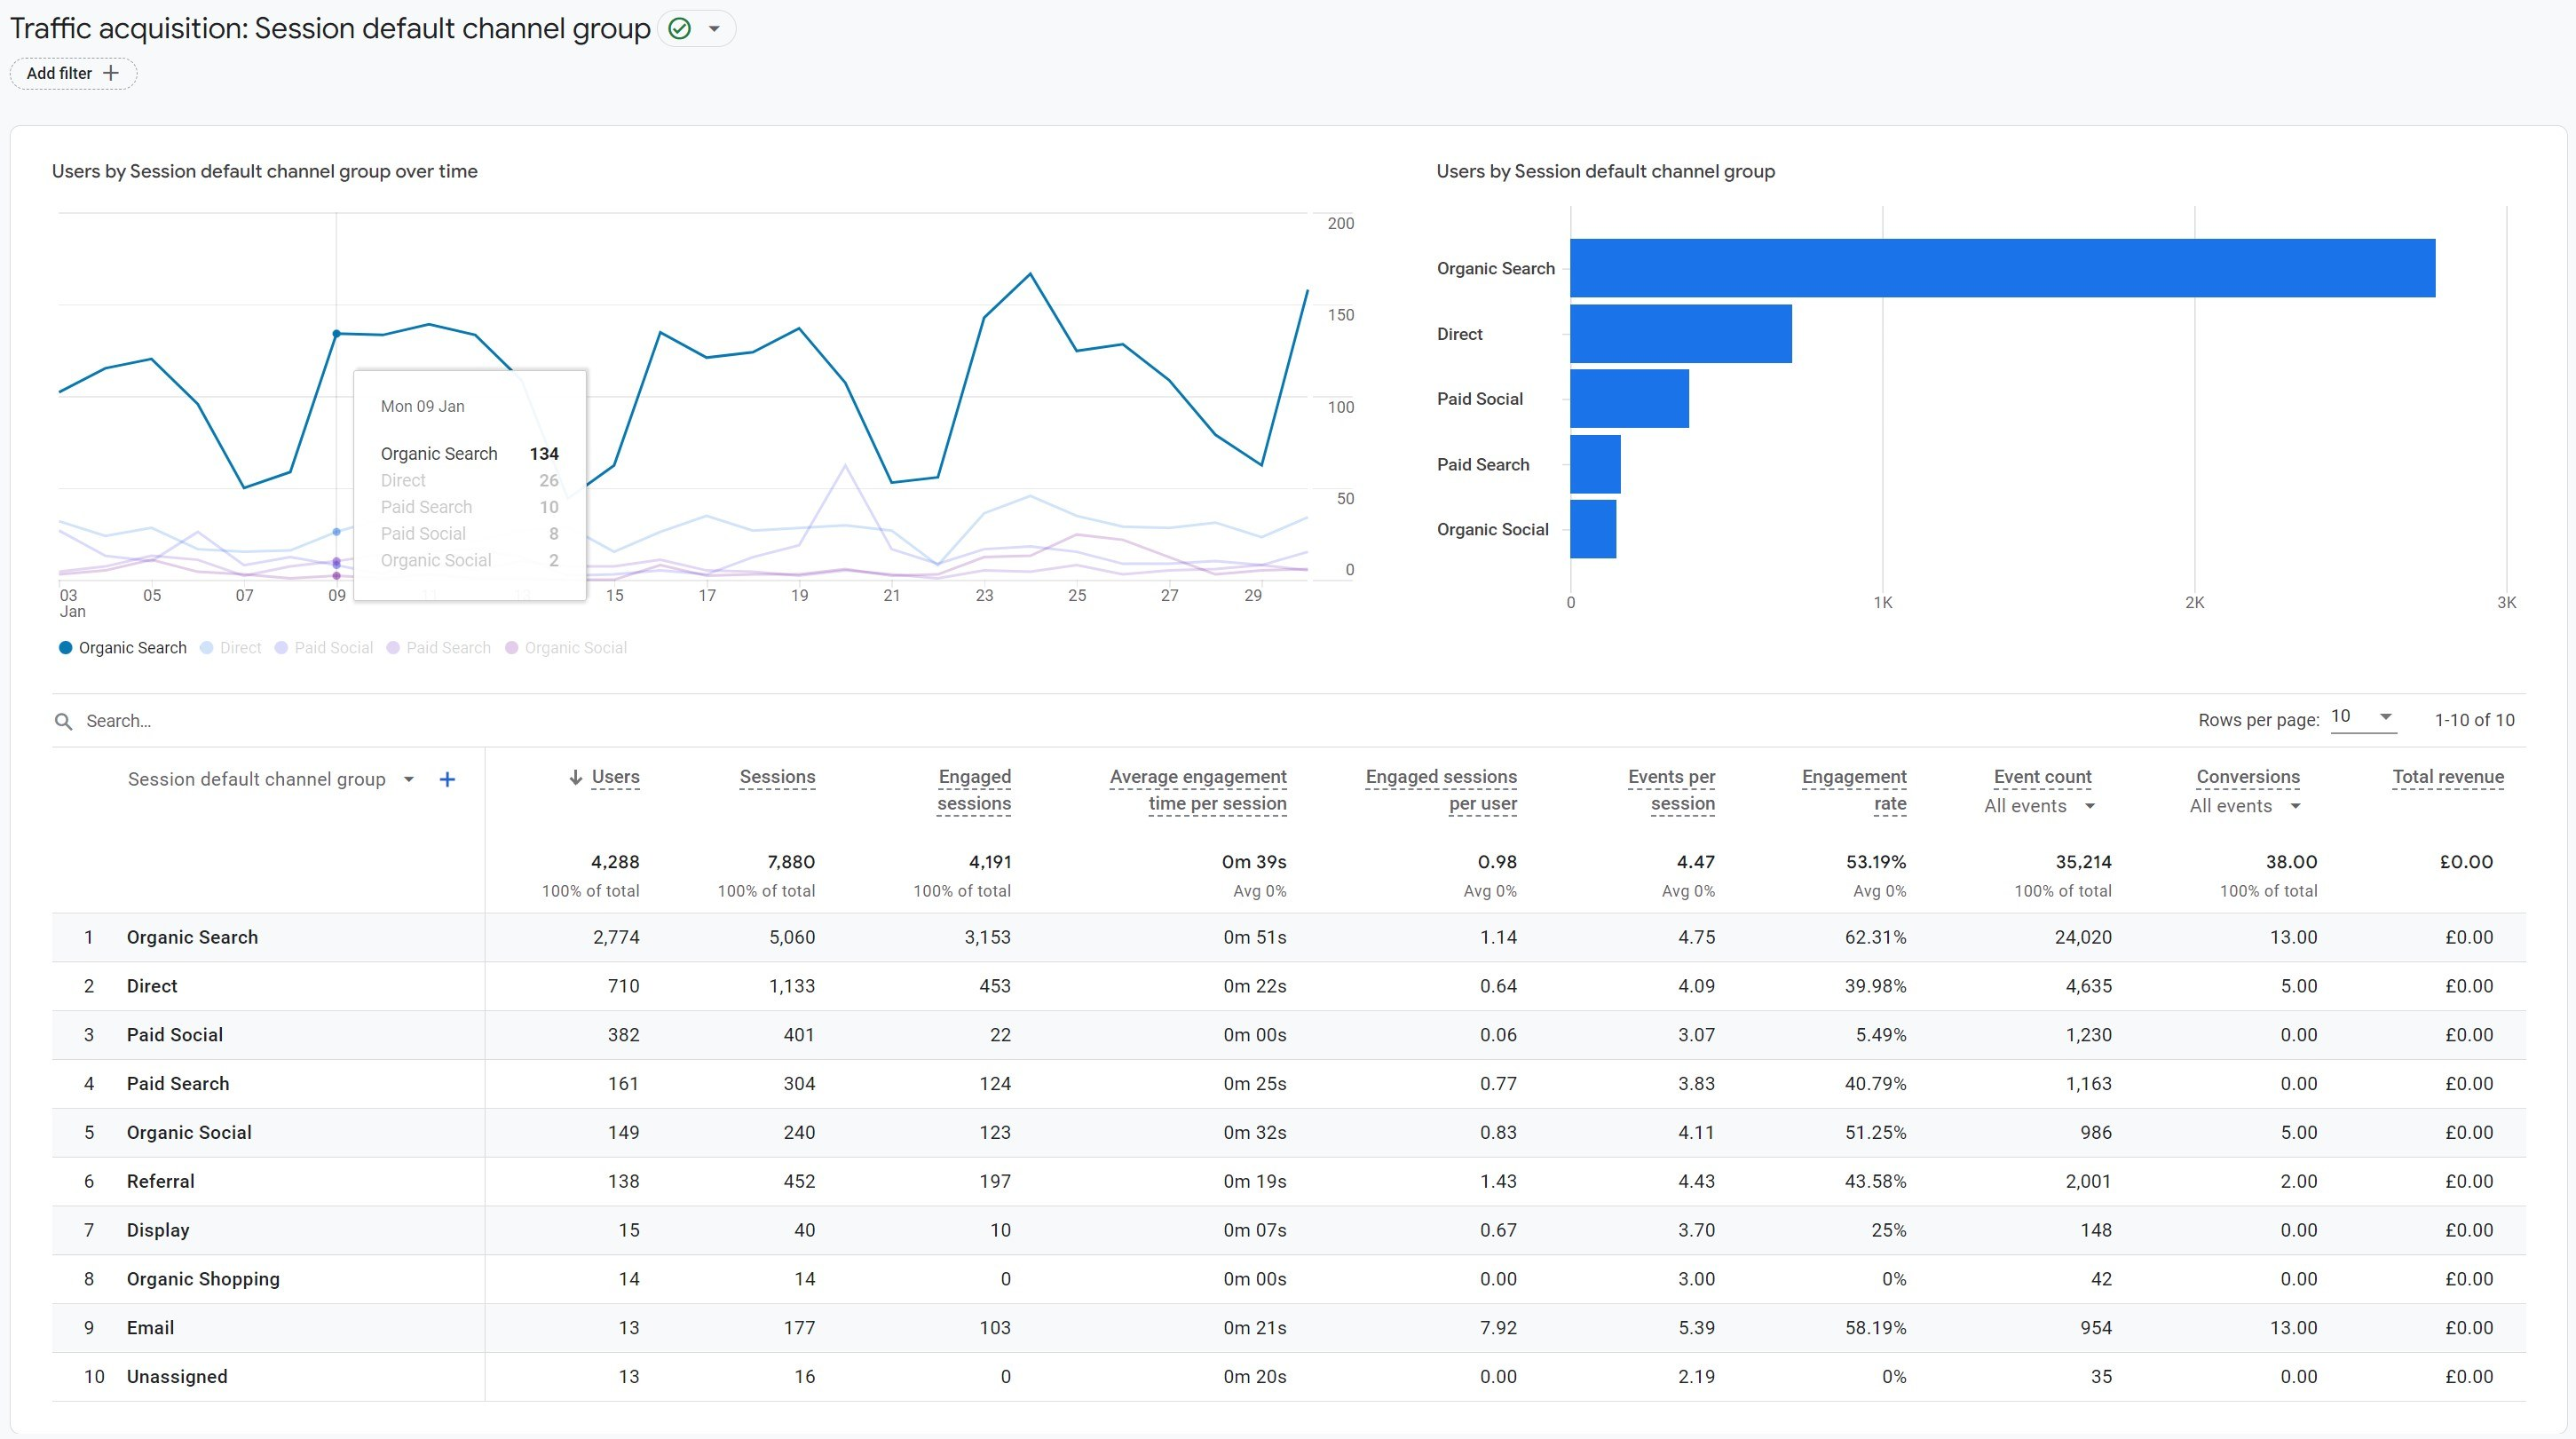
\includegraphics[width=1\textwidth]{problem-analysis/GA4-acquisition}
    \caption{\acrshort{ga4} session acquisition.
    }\label{fig:GA4-acquisition}
\end{figure}

Figure~\ref{fig:GA4-acquisition} shows an example of a session acquisition overview in \acrshort{ga4}~\cite{ga4-tips}.
This is one of the submenus in the dashboard, and it shows data on how users are acquired.
The top left graph shows the number of users acquired each day per channel group, and the top right graph shows the
total acquisition per channel group.
The list below breaks every channel group down into numbers, and it also shows user retention, engagement, and sales.
A channel group is a group of sources that a user can come from, such as organic search, direct link, paid
advertisement, and many more.
The main purpose of this overview is to show the manager if the marketing campaigns are effective and if the users are
then retained and engaged.

% textidote: ignore begin
\acrshort{ga4} has similar overviews for many other statistics that can be tracked, most notably being user engagement
and monetization.
% textidote: ignore end
User engagement shows how users interact with the website, such as how long they stay, how many pages they visit, and
how they navigate the site.
Monetization shows how the website makes money, such as how many products are sold, how much money is made, and how
many users are retained.

The disadvantages of~\acrlong{ga4} are that it's limited in what services it can integrate with.
It is designed for digital services, so it can't natively track physical goods.
This means that~\acrshort{ga4} cannot be used to solve the problem of tracking physical sales in a café.
The layout is also not very user-friendly, as it is designed for professionals that are used to working with data.
It can, however, be customized to be more user-friendly, but it requires some work.
% textidote: ignore begin
\acrshort{ga4} is a free service, but it also offers a paid option that allows for more features and better
support~\cite{ga4-360}.
% textidote: ignore end


    \section{Problem statement}\label{sec:problem-statement}

When meeting the owners of the Caf\'e, they established that they wanted to have a system that could provide them with
an overview of their sales, so they could make better decisions based on their data.
The data provided by the system would help optimize staff shifts, ensuring that the right number of employees are
scheduled for the right time of day.

Additionally, the caf\'e sells baked goods that need to be prepared in advance.
The system should enable the owners to analyze the sales data provided to see the customer traffic from previous weeks,
ensuring they can prepare the right amount of baked goods for the upcoming days.

With one of the owners not being very tech-savvy, we would need to make sure that the system is easy to use and
understand, so it is critical that we focus on the UX of the system.

This presents us with the following problem statement:
\begin{tcolorbox}[title=Problem statement]
    How can we design an application that provides the caf\'e owners with a comprehensive overview of their sales and
    facilitates better decision-making based on the available data, while ensuring that the system is intuitive and
    accessible for all users?
    %textidote: ignore begin
\end{tcolorbox}
%textidote: ignore end

    % textidote: ignore begin
\chapter{Method}\label{ch:method}
% textidote: ignore end

% textidote: ignore begin
\section{Technology}\label{sec:technology}
% textidote: ignore end

% textidote: ignore begin
\section{Development process}\label{sec:development-process}
% textidote: ignore end


    % textidote: ignore begin
\chapter{Problem solution}\label{ch:problem-solution}
% textidote: ignore end

% textidote: ignore begin
\section{Software requirement specification}\label{sec:software-requirement-specification}
% textidote: ignore end

% textidote: ignore begin
\section{Front end}\label{sec:frontend}
% textidote: ignore end

% textidote: ignore begin
\section{Back end}\label{sec:backend}
% textidote: ignore end


    % textidote: ignore begin
\section{Discussion}\label{sec:discussion-conclusion}
% textidote: ignore end

\subsection{Future Development}\label{subsec:future-development}
In this section, we will discuss the potential future development of the system.
The system has a lot of potential for future development, as it is a very basic implementation of the idea.
All the features that could be implemented in the future will be provided in a list below, with an expanded
explanation of each feature.

\begin{itemize}
    \item API Integration
    \item Faster response time
    \item Update an order
\end{itemize}

\noindent
\newline
\textbf{API Integration}

\noindent
The system could be more user-friendly if the system could be integrated with an API instead of uploading CSV files
to the system.
By having an API, the system would seamlessly update the data in the system, and the user would not have to upload,
making the system more automated and user-friendly.
The reason why this was not implemented is because of the~\acrshort{epos} system of the company, which does not provide
an API\@.

\noindent
\textbf{Faster response time}

\noindent
The system could be improved by having a faster response time.
The system is currently already fast enough for the user to use, but it could always be improved.
One of our would-haves was to have a faster response time, but we did have time to prioritize optimizing the system
for speed.
One way to improve the response time could be to optimize the reading and writing of the data in the system.
We could make asynchronous calls to reading the CSV files, which would make the system faster.

\noindent
\newline
\textbf{Update an order}

% todo: This could be moved to the next section and be a part of the software requirements evaluation
\noindent
The system could be improved by having the ability to update an order.
Currently, the system only allows the user to view the orders and then look at the details of the order.
The user cannot update the order, which could be a useful feature if something goes wrong with the order or is not
displayed correctly.
This feature was not implemented as it was not a priority for the systems' functionality, and it was labeled as a
could-have in Section~\ref{subsec:software-requirements-specification}.

\subsection{Software requirements evaluation}\label{subsec:software-requirements-evaluation}

In this section, we will evaluate the software requirements that were set at the start of the project.
We will look at both the tables of functional~\ref{tab:functional-requirements-specification}
and non-functional requirements~\ref{tab:non-functional-requirements-specification}.

\subsubsection{Must-haves}\label{subsubsec:must-haves}

In this section, we will evaluate the must-haves requirements.
Most of our must-haves have been implemented, and the system is functional.
That concerns uploading a csv file, creating a user, deleting a user, creating an order, getting a list of all orders
with a particular product ID and getting a list of all orders on a particular date.
\newline

\noindent
\textbf{Getting a list of all customers}\label{text:getting-a-list-of-all-customers}

\noindent
Although this requirement was a must-have, it has not been implemented.
The reason for this is that the requirement was not prioritized as highly as the other must-haves.
From the data we receive from the~\acrshort{epos} system, we do not have the information about the customers.
Therefore, we did not prioritize this requirement as highly as the other must-haves.
Even though this requirement was not implemented, the system is still functional without it and can be used by the
company. % todo: A little too much yapping here, maybe?
We have discussed this with the company, and they are aware that this requirement was not implemented.
But they are still satisfied with the system and the functionality it provides.

%textidote: ignore begin
\subsubsection{Should-haves}\label{subsubsec:should-haves}
% textidote: ignore end

In this section, we will evaluate the should-haves requirements.
A lot of the should-haves have been implemented, and the system is functional with them.
This section will only cover the requirements that have not been implemented.
\newline

\noindent
\textbf{Delete an order}\label{text:delete-an-order}

\noindent
Deleting an order was a should-have requirement, but it has not been implemented.
Once again, this requirement was not prioritized as highly as some other should-haves.
The reason for this is that it is not at all that important to the company to be able to delete an order.
As the company has an~\acrshort{epos} system that can already delete orders, so for that reason, it was not a priority
for the system to be able to delete orders.

\subsection{Final thoughts}\label{subsec:final-thoughts}

The system developed serves as a robust solution for the company.
Providing essential functionalities that the company can immediately use.
The initial implementation of the system effectively addresses several core requirements, such as handling the
csv files, authenticating users and displaying data.
These must-have features are crucial for the company to form a reliable operational framework, even if certain
lower-priority features were not implemented, like deleting an order.

The project holds significant potential for future development.
With the addition of API integration, the system could be more user-friendly and automated.
Similarly, faster response times could be achieved through methods like asynchronous data processing, which would
improve the user experience.

The system development journey has been a collaborative and iterative process, with essential features implemented
based on the practical needs of the company.
The system has been designed to be scalable and adaptable, with the potential for future development and expansion as
stated in Section~\ref{subsec:future-development}.

    % textidote: ignore begin
\section{Conclusion}\label{sec:conclusion}
% textidote: ignore end


    % Appendix
    \appendix

    % textidote: ignore begin
\chapter{Source Code Repositories}\label{ch:source-code-repositories}
% textidote: ignore end

Reference is made to our GitHub repositories:

    \subfile{process-analysis/process-analysis}

    % Bibliography
    \printbibliography[heading=bibintoc]
\end{document}
